\documentclass[11pt,a4paper]{ctexart}
\usepackage[margin=2.3cm]{geometry}
\usepackage{amsmath,amssymb}
\usepackage{booktabs}
\usepackage{graphicx}
\usepackage{xcolor}
\usepackage{caption}
\usepackage{enumitem}
\usepackage{longtable}
\usepackage[colorlinks=true,linkcolor=blue!50!black,urlcolor=blue!50!black]{hyperref}
\setCJKmainfont{Noto Sans CJK SC}
\setCJKsansfont{Noto Sans CJK SC}
\captionsetup{font=small}
\renewcommand{\arraystretch}{1.12}
\setlist[itemize]{leftmargin=1.4em,itemsep=0.15em,topsep=0.25em}
\setlist[enumerate]{leftmargin=1.5em,itemsep=0.15em,topsep=0.25em}

\title{\bfseries 张靖皋猫道动力频率复现：全程时间线\\
\large 从静力复核到扭转可达域——这到底是一个什么问题}
\author{时间线整理稿（证据均注出处；口述补充单独标记）}
\date{2026 年 8 月 27 日}

\begin{document}
\maketitle

\noindent\fbox{\parbox{\dimexpr\linewidth-2\fboxsep}{
\textbf{性质声明（not\_a\_scientific\_claim）}：本文是复现工作的时间线与问题定性记录，面向未参与此项工作的读者。全部日期取自 git 提交、运行目录时间戳（UTC）或文档自署日期；无法用文件核证、仅由当事人口述的条目以 ``◇'' 标出。本文不宣布复现成功，不修改任何已锁定结论。
}}

\vspace{0.5em}
\section*{一页版：这是什么问题}

一句话：\textbf{一份权威报告（附件 2--3 表 4--1）里的三个扭转频率，用公开图纸和审计部件反复算不出来；一个月后我们能证明的不是``我们算对了''，而是``在公开输入下它算不出来''——并且找到了为什么一个月才走到这一步。}

它由三层构成，从里到外：

\begin{enumerate}
  \item \textbf{物理层（已定案）}：双幅猫道的系统扭转被``摆式物理''钉在竖弯频率上
        （张力与质量的横向二阶矩同构），幅内滚转又被审计钢结构锁在 1~Hz 以上——
        0.08--0.17~Hz 之间不存在由公开部件客观装配出的独立扭转分支，而附件 TA1（0.0996~Hz）恰在此间。
        三条互相独立的计算路径（解析、降阶、10 万节点全模型）在三个不同日期
        撞上同一个地板（0.071--0.073~Hz）。要离开地板，需要每品门架约
        $10^4$~N·m/rad 量级的连接柔度——图纸中没有这个参数的出处。
  \item \textbf{方法层（卡住一切的墙）}：可用的扭转观测量只有三四个频率，
        未知参数至少七个（荷载分担 $\alpha$、张力质量比 $\beta$、钢丝绳切线 EA、
        门架节点刚度、通道接口柔度、塔顶支承、两幅索力差）。方程少于未知数，
        任何正向计算——解析也好、更大的有限元也好——都不能创造新信息。
        项目在这堵``可识别性墙''前停摆过一次（8 月 8 日），重启后又用五发全模型
        撞了一遍（8 月 26--27 日）。正确动作从头到尾只有一个：去测量，或去索取对方源模型。
  \item \textbf{组织层（为什么花了一个月）}：工作分成了互不通气的平行轨道。
        8 月 8 日解析轨已经写出钉扎定理和缺失柔度的量级，8 月 26 日的全模型战役
        对此毫不知情，从零重新发现；解析轨自己的第三代文档瞄准了一份来历不明的
        频率清单；没有任何人（人或 AI）持有``整合''这个角色。
        每条轨道内部都很严谨，加起来却不复利。
\end{enumerate}

对外的问题定性：\textbf{这不是求解器问题（各轨残差 $10^{-10}$ 量级），
不是执行力问题（消融纪律很好），而是``复现之争''在证据不完备时的标准形态——
它最终不是被算出来的，而是被证据链定性的：举证责任已转移到未公开的原始模型一侧。}

\begin{figure}[h]\centering
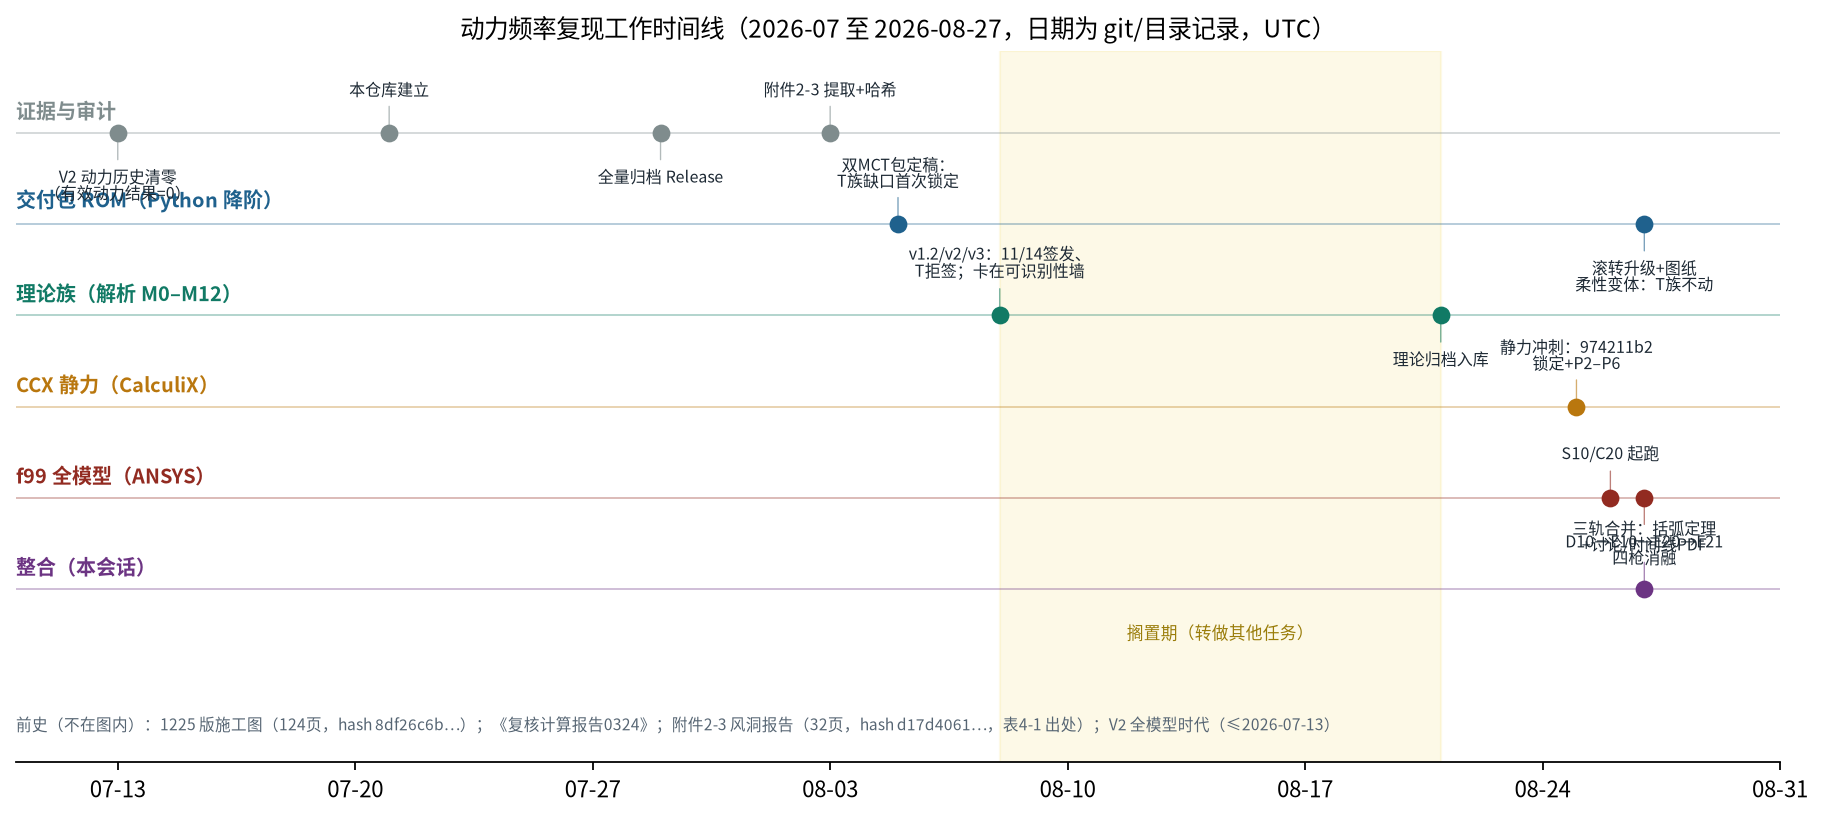
\includegraphics[width=0.99\linewidth]{assets/timeline_swimlane.png}
\caption{2026 年 7--8 月的六条泳道。黄色区间为搁置期。前史（1225 版图纸、0324 复核报告、附件 2--3、V2 全模型时代）在图下注记。}
\end{figure}

\section{时间线总表}

日期为 git 提交或运行目录时间戳（UTC）；``自署''指文档内落款日期；◇ 为口述补充。

\begin{longtable}{@{}p{2.1cm}p{2.2cm}p{7.2cm}p{3.4cm}@{}}
\toprule
日期 & 轨道 & 事件 & 锚点 \\
\midrule
\endhead
2025-12（版本号） & 外部文件 & 《猫道结构施工设计图》1225 版（124 页）：U 型螺栓、尼龙滚轮、销、抱箍等全部连接构造在此 & SHA-256 \texttt{8df26c6b\ldots} \\
0324（版本号） & 外部文件 & 《猫道结构复核计算报告 0324》——最早期的静力复核文件，后被解析轨用作交叉验证 & v1.2 文档引用 \\
（未署日期） & 外部文件 & 附件 2--3《施工猫道抗风性能研究报告》（西南交大，32 页，ANSYS R19.2）：表 4--1 十四行频率的唯一出处；\textbf{未附模型输入} & SHA-256 \texttt{d17d4061\ldots} \\
$\le$2026-07-12 & V2 全模型 & ``attachment23\_v2'' ANSYS 时代：静力证据、质量空间化审计 V2.0（963.811~t 空间化，误差 $10^{-13}$~t）、门架/横通道凝聚审计——后续一切模型的参数库在此建立；动力模态多次尝试 & main 分支 audit/* 存留 \\
2026-07-13 & V2 全模型 & \textbf{动力历史清零}：因共用 jobname 互相覆盖、结果无逐文件哈希绑定，全部历史动力结果按指令永久删除，``当前有效动力结果为 0 项''，求解脚本设为硬失败 & \texttt{DYNAMIC\_MODAL\_} \newline \texttt{DISABLED\_20260713} \\
2026-07-21 & 证据基建 & 本仓库建立（初始为桥梁 FEM 技能套件归档） & commit \texttt{77dac4a} \\
2026-07-22 & 证据基建 & 猫道自动化执行日志 + Skill Gate 保真度事故复盘入库——此前 CAD/FEM 技能链的失败被文档化 & \texttt{f5fccc7} \\
2026-07-29/30 & 证据基建 & 全量归档 Release \texttt{zhangjinggao-full-20260729}（含 1225 图纸与附件 2--3 原件） & 分支 \texttt{agent/archive-\ldots} \\
2026-08-01 & 证据基建 & 横向通道设计来源审计 & \texttt{6eb1e3f} \\
2026-08-03 & 证据基建 & Release 清点；附件 2--3 提取核证（哈希落档） & \texttt{b9a65e3} \\
2026-08-05 & ROM 轨 & \textbf{双 MCT 抖振复算包定稿}（◇双 MCT 拓扑为用户提出）：14 行正式配对首次锁定——非 T 主跨 $\pm2\%$，\textbf{T 族 $-28.2/-12.0/-8.5\%$，缺口第一次被干净隔离} & 包 README 自署 \\
2026-08-05 & 外部文件 & 《图纸汇总-2026.08.05.pdf》（175 页汇总版）生成，但不在 07-29 归档内，至今未随档核证 & 归档 delta 缺失 \\
2026-08-08 & 解析轨 & ◇用户提出``分层次分假设建理论模型''。v1.2（14 项模态独立验证：盲验协议、11/14 族签发 2.51\%、\textbf{扭转三行拒签}、反标量旋钮论证）、v2（谱序规律）、v3（M0--M12 阶梯：M3 钉扎定理、M7 预言缺失柔度 $0.65$--$1.9\times10^4$~N·m/rad）自署完成 & 三份文档自署 08-08 \\
2026-08-08 & 解析轨 & \textbf{停摆}：◇识别问题欠定（``四个频率、参数不够''）——即 M6 识别曲线``不能单凭频率唯一确定 $\alpha,\beta$''；用户转向其他任务 & v3 §6.4；◇口述 \\
2026-08-11 & （其他任务） & main 分支全天为扎青桥预应力工作——与口述``在忙别的''吻合 & \texttt{85ef043} 等 9 commit \\
2026-08-21 & 解析轨 & 理论族三代文档与可复现包归档入库（距完成已 13 天） & \texttt{08b30fa,33662f9} \\
2026-08-25 & CCX 静力轨 & \textbf{重启，从静力开始}：STEP$\to$CalculiX 管线、21/142 拓扑门禁、哈希主 deck \texttt{41fb3222}、ccx 2.21 静解、成形锁定 \texttt{974211b2}、P2--P6 与 DYN 子作业——一天冲刺 & 08-25 11:58--19:47 共 15 commit \\
2026-08-26 & f99 轨 & ◇链条由 GPT Pro 设计、豆包+Grok 4.6 执行。S10 基线与 C20（门架上销 ROTX）起跑 & 目录 \texttt{20260826T2211Z} \\
2026-08-27 & f99 轨 & D10（32 根物理下压索）07:54 → E10（通道刚臂 ALL$\to$UXYZ）12:58 → E20（刚臂换 COMBIN14 弹簧 $k{=}10^4$）15:04 → E21（$k{=}10^3$ 扫描）16:29。\textbf{前四枪 TA1 纹丝不动（$-26\%$）；E20 靠非出处弹簧抬到 $-15\%$} & 各运行目录时间戳 \\
2026-08-27 & ROM 轨 & 02:08 双 MCT 包入库；14:45 表 4--1 差异报告（锁定证据只分析）；16:16 滚转升级（双索组+双簇端口+质量空间化，含推导 PDF）；16:48 图纸连接核证 + drawing-soft 变体——\textbf{T 族横跨全部物理连接刚度区间漂移 $<0.7$ 个百分点} & \texttt{cfbf39e,09fb56d, 9e909b9,f20767c} \\
2026-08-27 & 整合 & 17:16 三轨首次合并：括弧定理成文、f99 对照、讨论 PDF；随后本时间线 & \texttt{e895c9d} 及本文 \\
\bottomrule
\end{longtable}

\section{三条计算轨道：互不知情，同一个地板}

三条路径使用完全不同的离散、不同的软件、由不同的会话在不同日期完成，事前互不引用：

\begin{table}[h]\centering\small
\begin{tabular}{lllrr}
\toprule
轨道 & 方法 & 完成日 & TA1 计算值 & 相对附件 \\
\midrule
解析（M0--M12 v1.2） & Ritz / 传递矩阵 & 08-08 & 0.0738 Hz & $-25.9\%$ \\
ROM（双 MCT 锁定版） & Python 降阶 13500 DOF & 08-05 & 0.0715 Hz & $-28.2\%$ \\
ROM（滚转升级 / 图纸柔性） & 双索组 + 双簇端口 & 08-27 & 0.0711 Hz & $-28.6\%$ \\
全模型（f99 S10--E10） & ANSYS 10.9 万节点 & 08-26/27 & 0.0733 Hz & $-26.4\%$ \\
全模型（f99 E20，非出处弹簧） & 通道 COMBIN14 $k{=}10^4$ & 08-27 & 0.0844 Hz & $-15.2\%$ \\
\midrule
附件 2--3 表 4--1 & ANSYS R19.2（输入未公开） & —— & 0.0996 Hz & —— \\
\bottomrule
\end{tabular}
\caption{TA1 跨轨道对照。三条独立路径钉在 0.071--0.073 Hz（摆式地板 $\approx$ VA1 $\approx2f^\ast$）；唯一离开地板的 E20 依赖图纸中不存在的弹簧刚度。}
\end{table}

\begin{figure}[h]\centering
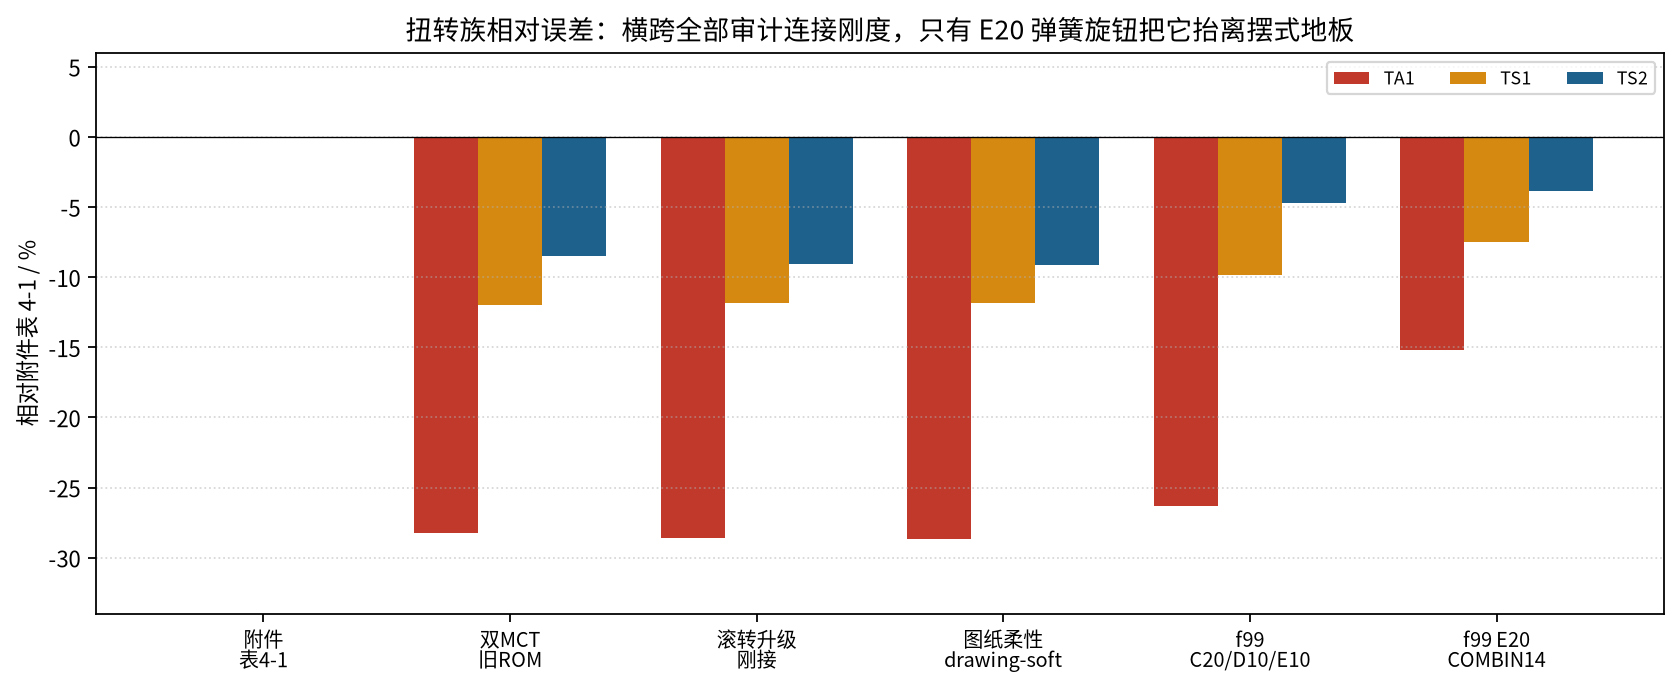
\includegraphics[width=0.95\linewidth]{assets/torsion_family_cross_model_error.png}
\caption{扭转族三行相对附件的误差：刚接、图纸柔性、全模型铰接链叠在同一条带上。}
\end{figure}

三轨还在另一个数字上汇合：\textbf{要把系统扭转从地板抬到附件值，所需门架连接柔度
约 $10^4$~N·m/rad/品}——解析轨 M7 于 08-08 正向预言（$0.65$--$1.9\times10^4$），
整合轨于 08-27 由附件频率独立反推（$0.9$--$1.5\times10^4$）。这个参数在 124 页
施工图的任何连接大样（M14 U 型螺栓、MC 尼龙滚轮、$\phi34$ 销、R76 抱箍）中都没有出处；
图纸连接实测方向恰恰相反——是``更软''而非``更硬''，而更软并不改变地板（钉扎与连接刚度无关）。

\section{问题的三层解剖（给旁观者）}

\subsection{物理层：不是算错，是不可达}

附件图 4-5 的 TA1 振型与全部三轨算出的系统扭转是同一形态（双幅反相竖向 X 交叉）。
争议只在频率。系统扭转的频率比由张力与质量的横向二阶矩之比决定，本结构两者同构，
比值 $\approx1$，于是扭转被钉在竖弯上——这是两行 Rayleigh 商可证的不变量，
与门架、销、下压索、通道刚臂的细节全部无关。f99 的五发消融是这个定理的
$10^5$ 节点实测版：改销、改下压、放开通道转角，TA1 的变化在 $10^{-5}$~Hz 量级。

\subsection{方法层：可识别性墙}

14 行参考频率里，扭转独立观测量只有 TA1/TS1/TS2 三个（加上近双根分裂的量级）；
未知参数至少七个。v1.2 在 08-08 已经把这堵墙写成了定理形式：对固定映射，
三行扭转要求的刚度修正为 $+82\%/+7\%/-27\%$——符号互相矛盾，
\textbf{任何单一标量旋钮在数学上不可能同时满足三行}。这个论证本该拦住 18 天后
E21 的``朝 0.0996 扫 $k$''，但没有人把它递过去。停摆的真实含义不是``算不动了''，
而是``计算已到达信息上限''——从这一刻起，唯一能推进问题的动作是获取新信息：
按 v1.2 §14.4 去测振型半波数、面层/门架顶相位、索力、节点柔度，或索取 R19.2 源模型。

\subsection{组织层：轨道不通气}

时间线上最贵的三段空转，全部源于状态不共享：

\begin{itemize}
  \item 08-08 解析轨已含钉扎定理（M3）与缺失柔度量级（M7），
        08-26 的全模型战役从设计上完全未引用——四发算例重新发现了纸上两行的结论；
  \item 解析轨第三代（v3）瞄准的 14 频清单 $\{0.0296,\ldots,0.1187\}$
        与已哈希核证的表 4--1 不符、与任何算例不符、出处只有``此前核对''四个字——
        v2 自己的附录早已警告``对照表系转录，归档应存原页和哈希''；
  \item 执行层（◇豆包+Grok）忠实执行了协议（门禁、清单、假设先行），
        但协议能传递、判断力不能：E21 目录里留着半改名的 E20 模板，
        而更重要的判断——``这笔弹簧储能物理上放在哪里''——没有人问。
\end{itemize}

一个月的直接代价，就是``整合''这个角色空缺的代价。它在 08-27 被补上之后，
全部既有材料在一天内合并成了定案。

\section{当前定案与遗留分叉}

\textbf{已定}（详见讨论稿与推导稿两份 PDF）：
非 T 主跨行 $\pm2\%$ 复现；T 族偏差是审计部件可达域之外的结构事实，
横跨全部物理连接刚度区间不动；附件 T 行依赖一个未公开、与图纸和摆式物理
不一致的隐含假设；举证责任在原始模型一侧。VS2（$-17\%$）与扭转通路解耦，
指向索系 EA/初张力口径，单列。

\textbf{遗留分叉——全部是取数据，没有一项是``再跑模型''}：

\begin{enumerate}
  \item 附件原始 ANSYS 输入（R19.2 源模型）——对方不给，则按举证转移写最终定案；
  \item v3 那份 $\{0.0296,\ldots,0.1187\}$ 清单的原页——一页纸决定 M0--M12
        第三代的谱序结论是否成立；
  \item 《图纸汇总-2026.08.05.pdf》175 页原件——核证通道数量（12/13/21 三种清点冲突）；
  \item 若有现场条件：v1.2 §14.4 的四级最小补测（振型 $\to$ 相位 $\to$ 索力 $\to$ 节点柔度）。
\end{enumerate}

\section{给后来者的三条规则}

\begin{enumerate}
  \item \textbf{先算可达域再开算例}：任何昂贵计算前，先用不变量（本例：二阶矩之比）
        判断目标是否在当前部件的可达域内；
  \item \textbf{禁止朝参考值扫参数}：新增刚度必须附能量出处说明，否则是标定不是复现；
  \item \textbf{目标清单必须带原页和哈希；``整合''必须是一个显式角色}——
        每条轨道收尾时向共享台账写入：已证定理、已否证机制、未决参数。
\end{enumerate}

\appendix
\section{证据索引}

\begin{itemize}
  \item 锁定配对与差异报告：\texttt{modal\_validation/gate\_corrected\_*}；
        \newline 分支 \texttt{cursor/table41-fable5-diff-d416} 之
        \newline \texttt{docs/TABLE41\_FABLE5\_DIFF.md}
  \item 理论修复与讨论（均在分支 \texttt{cursor/mct-torsion-theory-fix-d416}）：
        \newline \texttt{report/double\_mct\_torsion\_theory\_fix\_cn.pdf}
        \newline \texttt{report/double\_mct\_torsion\_discussion\_cn.pdf}
  \item 解析族三代：分支 \texttt{feat/catwalk-thirteen-theory-models} 之
        \newline\texttt{catwalk-theory/thirteen-mode-models/}
  \item 全模型链：分支 \texttt{f99-chain-closure} 之 \texttt{ultra\_runs/}
        （\texttt{frequency\_compare\_*.md}、各工况 \texttt{qa/*table41*}）
  \item V2 清零记录：main 之 \texttt{DYNAMIC\_MODAL\_DISABLED\_20260713.md}
  \item 关键哈希：1225 图纸 \texttt{8df26c6b\ldots}；附件 2--3 \texttt{d17d4061\ldots}；
        APDL 源 \texttt{ba9d062e\ldots}；CCX 主 deck \texttt{41fb3222\ldots}
  \item ◇口述补充（未经文件核证）：理论分层与双 MCT 拓扑为用户提出；
        链条由 GPT Pro 设计、豆包与 Grok 4.6 执行；08-08 停摆原因为识别欠定。
\end{itemize}

\end{document}
